% !TeX root = ../main.tex

% Background
% Identify the necessary background
% Explain the background info in sufficient details
\chapter{Background}\label{chapter:background}
In this chapter, we're going to dive into the basics of how emulators work and why they're important.
Understanding the process behind emulators is key to figuring out why certain errors occur.
Specifically, we'll explore how emulators convert binary code so it can run on different types of computers.
This conversion process is quite important because mistakes in it are often the source of the errors we're trying to fix.
Knowing how this translation works helps us get to the root of the problem.

Next, we'll discuss our primary emulator targets.
While the reproducer and the verifier need generic input, there are two main emulators we're concentrating on.
We'll provide some insight into these emulators, including how they function and the specific techniques they use.

Lastly, we'll look into the execution methods used by the verifier.
These methods are significant because the reproducer relies on data obtained through them.
Understanding these execution strategies is essential for understanding how the reproducer turns this data into programs that trigger bugs.

\section{Binary Translation}
Binary translation is an advanched technique that enables the execution of code compiled for one CPU architecture (the guest architecture) on a different CPU architecture (the host architecture).
This process involves analyzing and converting the binary instructions from the guest architecture into a form that can be understood by the host architecture. 

Binary translation is particularly useful in scenarios such as software emulation, where applications or entire operating systems designed for one type of hardware need to run on an entirely different type of hardware.
For instance, running a binary compiled for ARM architecture on an x86-based system would be impossible without any change. This necessitates binary translation.
The technique is quite important in achieving compatibility across diverse hardware platforms, enabling a broader software reach and facilitating the preservation of legacy software on modern hardware.

\subsection{Dynamic Binary Translation}
Dynamic translation, a subset of binary translation, involves translating binary code at runtime, as the program executes.
This approach contrasts with translating the entire program, all at once, before execution begins.
Dynamic translation offers the advantage of adaptability as it can optimize the translation based on the actual execution path of the program, which may vary from run to run.

This method is especially usefull in emulating complex software where it's impractical to predict all possible execution paths in advance.
Dynamic binary translators tend to work on basic blocks and they often incorporate a cache to store recently translated instructions, reducing the overhead of re-translating those instructions on subsequent executions. 
This caching mechanism is a key factor in mitigating the performance penalty associated with runtime translation, making dynamic translation an efficient and versatile approach for system emulation and virtualization environments.
\begin{figure}[ht]
    \centering
    
\includegraphics[width=0.2\linewidth]{figures/placeholder}
    \caption{Dynamic Binary Translation}
    \label{fig:dynamic_binary_translation}
\end{figure}

\subsection{Static Binary Translation}
Static translation, in contrast to dynamic translation, involves converting the entire binary code from the source architecture to the target architecture before execution begins.
This approach allows for thorough analysis and optimization of the translated code, potentially leading to better overall performance for the translated application.
However, static translation faces challenges in handling dynamic aspects of program execution, such as just-in-time compilation or self-modifying code, which are better managed by dynamic translation techniques.
Static translation is well-suited for scenarios where the complete binary image is available and the execution environment is stable and predictable.
\begin{figure}[ht]
    \centering
    
\includegraphics[width=0.2\linewidth]{figures/placeholder}
    \caption{Static Binary Translation}
    \label{fig:static_binary_translation}
\end{figure}

\section{QEMU}
\ac{QEMU} is a well known free and open-source emulator and a virtualizer. 
At its core, \ac{QEMU} employs dynamic binary translation which lets the host machine run programs belonging a different architecture.
Complementing this capability is the \ac{TCG}, an integral part of \ac{QEMU} that dynamically generates native code for the host CPU.
As shown in \ref{fig:qemu_tcg} the \ac{TCG} is used to translate a foreign ISA into the host's architecture.

\begin{figure}[ht]
    \centering
    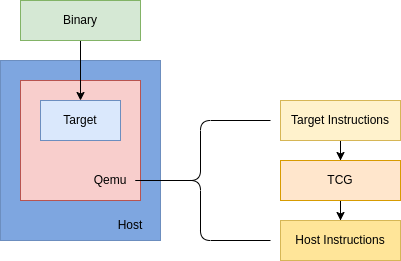
\includegraphics[width=0.8\linewidth]{figures/Qemu_TCG}
    \caption{\ac{QEMU} translation process with \ac{TCG}}
    \label{fig:qemu_tcg}
\end{figure}

\section{TCG}
\ac{TCG} \cite{qemu_tcg} which began as a generic backend for a C compiler was later improved upon be both portable and efficient, allowing \ac{QEMU} to quickly translate the guest instructions into a form that can be directly executed by the host machine, thereby improving the speed and efficiency of the emulation process.
This combination of dynamic binary translation and the flexibility of \ac{TCG} enables \ac{QEMU} to provide a high-performance and versatile solution for system emulation.
Thanks to the flexibility of the \ac{TCG}, many different architectures are supported by \ac{QEMU}.

These include \cite{qemu_arch}:
\begin{itemize}
    \item Arm
    \item MIPS (little endian)
	\item PPC
	\item RISC-V
	\item s390x
	\item SPARC
	\item x86
\end{itemize}

\section{Arancini}
Arancini is a project from the Systems Research Group at the \ac{TUM}.
It builds on the knowledge gained from two earlier projects: Lasagna which translates any x86 program statically to an Arm ISA and Risotto which emulates x86 program dynamically on an Arm machine.
Like these previous projects, Arancini focuses on making x86 programs work on Arm, but it also adds support for RISC-V systems.
It uses a combination of LLVM, a well-known toolkit for building compilers, and its own custom translation technology to achieve this.

\section{Concrete Execution}
Concrete execution refers to the traditional method of running programs where, the program operates on actual, specific input values to produce outputs.
In this execution model, the program's instructions are carried out step by step, with each operation performed using concrete data values provided at runtime or predefined in the program. 
This method is straightforward and mirrors how programs are executed in real-world scenarios, making it intuitive and easy to understand. 

Concrete execution is particularly useful for debugging, as it allows developers to trace the exact sequence of steps a program takes with a given set of inputs, observing the program's behavior and output directly.
However, its reliance on specific inputs means that concrete execution can only explore one path through the program at a time, limiting its ability to uncover issues that may arise with different inputs or in untested execution paths.

\section{Symbolic Execution}
Symbolic execution, on the other hand, abstracts away from concrete input values, instead treating inputs as symbolic variables that can represent multiple possible values simultaneously. 
This approach allows the program to be executed in a way that explores multiple execution paths in a single run, by considering all the possible values that the symbolic variables might take. 
Symbolic execution builds a mathematical model of the program's execution paths, using symbolic expressions to represent the outcome of computations and decisions based on the symbolic inputs. 
As you can see in the figure \ref{fig:sym_tree} every possible branching instruction adds a new path.
\begin{figure}[ht]
    \centering
    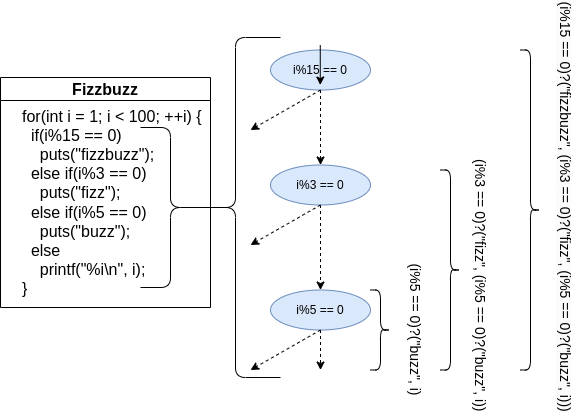
\includegraphics[width=0.8\linewidth]{figures/sym_trans}
    \caption{An example of a branching code in a tree}
    \label{fig:sym_tree}
\end{figure}

This model can then be analyzed to identify potential bugs, security vulnerabilities, or performance issues across a wide range of input conditions without having to enumerate and test each one individually. 
While powerful, symbolic execution is computationally intensive and can face challenges like path explosion, where the number of possible execution paths grows exponentially with the complexity of the program.



\section{Concolic Execution} 
Concolic execution, a hybrid approach combining concrete and symbolic execution, aims to mitigate some of the limitations of both methods. 
In concolic execution, the program is run with specific concrete input values, like in concrete execution, but at the same time, it tracks symbolic constraints derived from the execution path taken. 
By analyzing these constraints, concolic execution tools can systematically generate new concrete inputs that will explore different paths through the program, combining the depth of symbolic analysis with the actual values from concrete execution.

This approach allows for more efficient exploration of the program's execution space, making it possible to uncover subtle bugs or vulnerabilities that might not be evident through conventional testing. 
Concolic execution has proven particularly useful in software testing and verification, providing a balance between the thoroughness of symbolic execution and the directness of concrete execution.

\section{Miasm}
Miasm \cite{miasm} is a framework primarily designed for reverse engineering and binary analysis.
It features tools such as disassembler and a symbolic execution engine.
The framework operates by taking advantage of the features of the symbolic execution engine, where binary code is interpreted in terms of symbolic expressions rather than concrete values.

This symbolic approach allows the theorem solver to evaluate the logical and mathematical properties of the code, solving constraints and proving or disproving theorems about the code's behavior under various conditions.
It also paints a clear picture about the transistion of the register and memory states between instructions and basic blocks.
The produced symbolic expressions are invaluable when comparing different states as they can pinpoint the expected changes and the actual ones.

\section{Focaccia}
Focaccia is a specialized verifier program designed with the goal of assessing the accuracy of emulators.
It uses concolic execution to collect data from a binary and comapare it with an emulator's log.
At its core, Focaccia works by comparing these two data sets.
The first set comprises the memory and register values obtained during a test run on actual hardware, which serves as the benchmark or 'oracle' for expected outcomes. 
The second set involves the detailed log produced by the emulator during its operation, which records various actions including register modifications, memory writes, and the current position of the \ac{PC}.
These logs are integral to the verification process as they provide a sequential record of the emulator's behavior, which lets Focaccia find the cutoff point where it starts to behave differently.

The verifier uses the Miasm reverse engineering framework for breaking down the original binary code into symbolic expressions for each operational step, transforming the instructions into a more abstract and analyzable form.
These symbolic expressions represent the ideal state changes that should occur step by step according to the software's design.
Focaccia then does a detailed comparison between these  symbolic expressions and the actual state changes recorded in the emulator's log.

This comparison is the focal point of the verifier as it highlights any discrepancies between the expected behavior (as defined by the symbolic expressions) and the actual behavior observed in the emulator.
Discrepancies signal potential bugs in the emulator, indicating that the emulator's reproduction of hardware behavior is not entirely accurate.


